% -*- coding: utf-8 -*-
%%
%%  本模板可以使用以下两种方式编译:
%%     1. PDFLaTeX
%%     2. XeLaTeX [推荐]
%%  注意:
%%    1. 在改变编译方式前应先删除 *.toc 和 *.aux 文件,
%%       因为不同编译方式产生的辅助文件格式可能并不相同。

\documentclass{cumcmart}
%\documentclass[nocover]{cumcmart}%%%切换到无封面的版本,有些区域不允许前面的承诺页用pdf格式,可以用此去掉。



\begin{document}


\title{基于差分方程和元胞自动机的交通阻塞模型}

\xuanti{A}
%\school命令用于在承诺书上显示学校名称。按要求,此处应填写全称
\school{上海交通大学}
%以下命令分别显示队员及指导教师姓名
\numbers{2010888}%参赛报名号
\authorone{印定豪}
\authortwo{赵鹭天}
\authorthree{赵方舟}
\advisor{数模指导组}

%\theyear{2010}

\theday{16}%填写当月的具体日期

\maketitle
\begin{cnabstract}%此处没有采用sbstract命名,是为了将来如果要加入英文摘要时扩展的方便
针对题目要求,我们建立了两个预测事故发生后阻塞道路上的交通情况。分别利用了两个不同的模型,对交通状况与事故持续时间,车辆通行量以及上游车来源量进行了估计与研究。

第一个模型是差分方程模型。该模型对下一个步长内进入的车辆进行了估计。利用从视频内统计的数据,我们给出了车流量近似表达式,同时提出一个带随机量的差分方程。通过解这样一个方程,我们得到了一个震荡增加的随机函数。该模型的特点是解的速度快,解的趋势较好把握,同时能够得出符合实际的结论。

第二个模型是元胞自动机模型。考虑第一个模型不显然性,我们利用元胞自动机简明易懂的特点,将汽车看成有规律,坚固且只有有限个状态(速度)的物体。利用生活中的一些规则,将其数学化后进行计算机实验。我们同样利用了视频里的统计数据,对其进行计算后得到一系列队伍长度与各个参数的关系。该模型以随机性强,符合现实情况。虽然同样不能给出显示表达式,但是我们能够通过动画演示将其具现化。

在文中将两种模型进行了多次比较。利用视频里的一段堵车的摄影,我们分别用两种模型平均值的趋势,得到。同时我们也利用一些相同的数据代入,计算车流到达路口时时间长度。最后,我们得出两种模型其实是对一类问题的两种表述这一结论,从而增加了对同一类问题的求解方式。


\cnkeywords{差分方程,元胞自动机,交通阻塞模型,数值模拟}
\end{cnabstract}

\newpage
%\tableofcontents\newpage%增加目录,要不要都可以。不想要的话,就在本行前加“%”(英文的百分号)


\section{问题重述}
在城市道路交通中难免会由于交通事故、修路活动、违章停车导致的车道占用现象,严重影响道路的通行能力。本文通过分析研究同一路段同一截面两次交通事故的车流通行状况监控录像,建立了能够模拟出现车道占用现象后车流通行状况的几个模型,希望能够对交通管理部门正确引导交通、优化由于施工、停车导致的车道占用方案提供理论依据。

我们需要研究的问题有:找到一个能够衡量道路通行能力的指标,通过观察记录监控视频中的车辆通行状况来找到事故发生后道路通行能力随时间的变化规律;分别统计记录事故发生在不同位置时道路的通行状况,来找出导致道路通行能力不同的因素;通过建立模型来模拟事故发生前后车流通行情况来找出车辆不同的事故持续时间、不同的上游车流量以及不同的道路实际通行能力对排队长度的影响;利用构建的模型来模拟上游路口距离事故发生地点140米、下游需求量不变、事故发生不撤离为条件下车辆排队队尾何时到达上游路口。

\section{道路实际通行能力问题研究}
\subsection{现象观察}
观察附件中视频1和视频2两份文件,我们看到问题研究的对象是一条三车道的城市道路,每条车道宽度均为3.25m左右,事故发生位置距离上游第一个路口的距离和距离下游第一个路口的距离均为240m;同时,事故发生位置到上游第一个路口之间有两个小区入口,会有随机的流量较小的车流进出。

在视频的开始,道路没有事故发生,车辆均行驶通畅,没有发生拥堵现象。之后事故发生,完全的占据了两条车道,视频1中事故占据了车道二和车道三,视频2中事故占据了车道一和车道二;与此同时我们看到,道路实际通行能力显著下降,车辆在行驶到接近事故位置时均选择减速缓行,较靠近事故位置车辆的减速,也传递到了较远离事故位置的车辆,直观上可以看到整体通行速度下降,但尚未出现拥堵现象;事故发生一段时间后,由于上游来车流量的阶段性上升以及事故发生位置车辆的滞留,出现了明显的拥堵现象,排队长度一度达到120m左右,但拥堵的排队现象往往在排队产生后的几分钟内慢慢消解,整体路况恢复基本正常;在不断出现阶段性的拥堵和正常通行后,事故移除,路况恢复正常,通行能力恢复正常,排队通过事故位置的车流得到释放,车流量接近正常状态下实际通行能力,经过短时间的车流释放后,道路路况恢复正常。

\subsection{问题分析}
我们的研究问题是在两段视频中,事故发生所造成的道路实际通行能力发生的变化。首先我们要明确道路实际通行能力的概念内涵。实际通行能力刻画的是在给定道路条件下,道路所能通过的最大交通流量;最大交通流量可以通过理论估计,也可以通过实际测量。

我们首先考虑通过实际测量来确定实际通行能力。实际通行能力刻画的是可能的最大交通流量,因此实际的交通流量只有当它达到饱和的时候,才能反映实际通行能力。在研究问题,道路存在两种基本状态,一是有事故车辆占用车道的状态,二是无事故车辆占用车道的状态。

通过对视频的观察我们可以大致确定道路实际通行能力的变化趋势。事故发生,道路被事故车辆占用,此时道路实际通行能力大幅下降,而在事故发生到移除的这段时间内,道路条件不发生变化,因此实际通行能力不变;事故移除后,被占用车道恢复通畅,此时道路条件和事故发生前完全一样,因此道路实际通行能力将上升恢复到事故发生前的状态。基于这样的分析,我们只需要确定有事故车辆占用车道和无事故车辆占用车道两种状态下的道路实际通行能力。

在有事故车辆占用车道的状态下,观看视频我们发现,出现过多个周期的道路饱和状态,即道路已经发生拥堵的状态,这种状态下的交通流量可以近似认为是该状态下的道路实际通行能力。因此要测量有事故车辆占用车道状态下的实际通行能力,我们需要采集在事故发生之后事故位置横截面的交通流量数据。
\begin{figure}
\centering
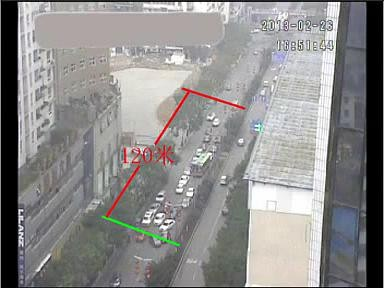
\includegraphics[width=.6\textwidth]{fig1}
\caption{发生事故时车流饱和状态图示}
\end{figure}


而对于没有事故车辆占道的情况,由于视频没有相应的道路饱和时刻,我们采取理论分析的办法估计这种状态下道路的实际通行能力。


\subsection{数据采集}
由于不同种类的车型对于道路交通压力的贡献大小不一样,并且不同种类的车型运输的客运量也不同,我们对过往各个路口与事故横截面的车辆进行了分类记录。由于小轿车与面包车的体积与运输能力比较相近,我们将小轿车与面包车归为一类车。我们将所有车型分成了三类,分别为小轿车与面包车、大客车、电瓶车。我们在网络上查找了不同车型对应的标准车当量($ {pcu}$),通过统计计算单位时间内通过道路某一横截面的标准车当量的多少来确定道路的通行能力。

我们通过观看视频,人工计数的方法,统计了视频中特定时间段中,通过事故位置横截面的三种类型的车辆数目。

\subsubsection{不同车型所对应的标准车当量(pcu)$^{\mathbf{[1]}}$}
\begin{table}[h]
\centering
\begin{tabular}{|c|c|}
\hline
\bf 车型&\bf 标准车当量(pcu) \\
\hline
小轿车/面包车&
1 \\
\hline
大客车&
3.5 \\
\hline
电瓶车&
0.5 \\
\hline
\end{tabular}
\caption{ 不同车型对应标准车当量}
\end{table}

\subsubsection{视频1-事故车辆占用车道二与车道三时的实际通行能力}
我们选择了视频1中道路出现显著饱和状态的视频片段,记录下了该片段的起始和结束时间点,计数了这段时间内的交通流量,统计结果如下。
\begin{table}[h]
\centering
\begin{tabular}{|c|c|c|c|c|c|c|c|}
\hline
&开始时间&结束时间&小轿车/面包车&大客车&电瓶车&总pcu&总时间 \\
\hline
1&16:42:32&16:44:47&27&5&5&47&0:01:45 \\
\hline
2&16:47:58&16:49:38&33&1&8&40.5&0:01:40 \\
\hline
3&16:52:42&16:56:05&91&4&17&113.5&0:05:23 \\
\hline
总数&&&151&10&30&201&0:08:48 \\
\hline
\end{tabular}
\label{tab3}
\caption{视频1中道路实际通行能力统计}
\end{table}
\subsubsection{视频2-事故车辆占用车道一与车道二时的实际通行能力}
\begin{table}[h]
\centering
\begin{tabular}{|p{33pt}|l|l|l|l|l|l|l|}
\hline
&开始时间&结束时间&小轿车/面包车&大客车&电瓶车&总pcu&总时间 \\
\hline
1&17:41:46&17:43:19&39&3&11&55&0:01:33 \\
\hline
2&17:50:04&17:53:55&69&4&31&98.5&0:03:51 \\
\hline
3&17:54:51&17:57:06&42&6&26&76&0:02:15 \\
\hline
4&17:58:51&18:01:08&36&5&11&59&0:02:17 \\
\hline
5&18:02:06&18:03:34&29&4&3&44.5&0:01:28 \\
\hline
总数&&&215&22&82&333&0:11:24 \\
\hline
\end{tabular}
\caption{视频2中道路实际通行能力统计}
\end{table}
\subsection{道路实际通行能力计算}
\subsubsection{有事故车辆占道时最大通行能力的估计}
我们在视频1和视频2中分别找到了3段道路明显饱和的时间和5段道路明显饱和的时间。我们分别计算了在这3个饱和时间段和5个饱和时间段内通过的标准车当量的总数以及这些时间段的总时长。用通过的标准车当量的总数除以总时长,这样就计算出了两种不同位置的事故条件下道路单位时间内通过的标准车当量,也就是道路的实际通行能力。

\begin{table}[htbp]
\centering
\begin{tabular}{|c|c|c|}
\hline
 &\textbf{视频1}&\textbf{视频2} \\
\hline
\textbf{标准车当量总数(pcu)}&201&333 \\
\hline
\textbf{总时长(h)}&0.147&0.190 \\
\hline
\textbf{实际通行能力(pcu/s)}&0.3805&0.4867 \\
\hline
\end{tabular}
\label{tab5}
\caption{不同车道来车流量统计}
\end{table}

\subsubsection{事故车辆占道时最大通行能力的估计}
在无事故车辆占用车道的状态下,因为道路上只是不时地来车,道路上的车流通行量显然没有达到道路的实际通行能力。所以,我们只能用理论来估计无事故车辆状态下,道路的实际通行能力。

根据文献(信号灯控制下的交通流模型)中的分析我们可以得到道路的通行能力$ {q}$与道路上的车辆密度$ {\rho
}$、车辆首尾相接时形成堵塞的最大密度$ {\rho
}_{ {m}}$以及车辆密度接近时车辆的最大行驶速度$ {v}_{ {m}}$存在以下关系$^{[2]}$:
\[
 {q(\rho )=} {v}_{ {m}} {\rho (1-}\frac{ {\rho
}}{ {\rho }_{ {m}}} {)}
\]
$ {q}$为关于$ {\rho
}$的二次函数且二次项系数小于,所以,当$ {q(\rho
)}$的导数等于时$ {q(\rho )}$取到最大值。
\[
\frac{ {dq(\rho )}}{ {d\rho
}} {=} {v}_{ {m}} {(1-}\frac{ {2\rho
}}{ {\rho }_{ {m}}} {)}
\]
$ {\rho =}\frac{ {\rho
}_{ {m}}}{ {2}}$时$ {q}$取最大值。所以,只要估算出车辆首尾相接时形成堵塞的最大密度$ {\rho
}_{ {m}}$以及车辆密度接近时车辆的最大行驶速度$ {v}_{ {m}}$,就能够估算出道路畅通时的最大通行能力。

我们需要估算的道路最大通行能力以$ {PCU/s}$为单位,所以我们在估计最大密度$ {\rho
}_{ {m}}$时采用的单位是$ {PCU/m}$,估计最大行驶速度$ {v}_{ {m}}$时采用的单位是$ {m/s}$。

由于电瓶车的最大行驶速度远低于小轿车和大客车,电瓶车难以形成首尾相接的阻塞,并且电瓶车对于总通行量的贡献较少,我们在估计最大通行能力时忽略了电瓶车的影响。
\subsubsection{$\rho_{m}$的估计}
对于不同的道路,车辆首尾相接形成堵塞时车辆的最大密度不同,所以估计这条道路上堵塞车辆的最大密度的最好方法是观察分析视频。

我们在视频1中找到了四个车辆形成首尾相接的阻塞的时刻,我们分别统计了这四个时刻首尾相接排队的小轿车数量和大客车数量,并利用道路隔离栏上的路灯杆作为标度估计了排队的长度,记录数据如下:
\begin{table}[h]
\centering
\begin{tabular}{*{5}{|c|}c|}
\hline
& 小轿车/面包车& 大客车& $ {PCU}$& 排队长度(m)& 车密度$ {\rho}_{ {m}}$ \\
\hline
1& 21& 1& 24.5& 80& 0.3063 \\
\hline
2& 20& 2& 27& 80& 0.3375 \\
\hline
3& 23& 1& 26.5& 80& 0.3313 \\
\hline
4& 24& 2& 31& 90& 0.3444 \\
\hline
平均& & & & & 0.3299 \\
\hline
\end{tabular}
\caption{不同车道车流量百分比统计}\label{tab6}
\end{table}

我们对四次采样得到的最大密度$ {\rho
}_{ {m}}$取了平均值以减小估算误差,估计这条道路上堵塞车辆的最大密度约为
$0.33 pcu/m$。


\subsubsection{$v_m$的估计}
因为达到车辆行驶最大速度的条件为车辆密度接近与,我们在视频中事故发生前选出了三段整条道路上车数小于2的片段,并对这三段视频中走在最前面的车的车速进行了估测。

我们分别利用路灯杆作为标尺,利用屏幕右上角的秒表读取时间,得到了三辆作为采样对象的汽车的速度。根据视频中出现的120标记大约有三个路灯杆间距的长度,我们估算第6个路灯杆到第2个路灯杆之间的距离大约有160m。

于是,我们便估计${v}_{{m}}$的数值大约有22.8m/s。
\begin{table}[h]
\centering
\begin{tabular}{|c|c|c|c|c|c|}
\hline
车辆& 经过第6个路灯杆的时间& 经过第2个路灯杆的时间& $ {\Delta t}/$s& 距离(m)& 速度(m/s) \\
\hline
1& 16:39:14& 16:39:22& 8& 160& 20 \\
\hline
2& 16:40:09& 16:40:16& 7& 160& 22.8 \\
\hline
3& 16:41:07& 16:41:14& 7& 160& 22.8 \\
\hline
\end{tabular}
\caption{等效实际通行能力计算}
\label{tab7}
\end{table}


估算好$ {\rho
}_{ {m}}$与$ {v}_{ {m}}$后,我们就可以计算道路畅通时的最大通行能力了。
\[
 {q}_{ {m}} {=q}\left( \frac{ {\rho
}_{ {m}}}{ {2}}
\right) {=}\frac{{ {v}_{ {m}} {*\rho
}}_{ {m}}}{ {4}} {=}\frac{ {22.8*0.33}}{ {4}} {\approx
1.9pcu/s}
\]
现在我们可以回答第一个问题。在事故发生后,道路实际通行能力由正常状态下
$ {1.95pcu/s}$ 下降到
$ {0.3805pcu/s}$,之后在事故移除后,道路实际通行能力上升恢复到正常水平,即$ {1.95pcu/s}$。

\subsection{不同事故位置影响的分析}

在观察视频的过程中,我们主要发现了两种因素可能会使得事故发生的位置不同时,道路的通行能力不同:


\begin{enumerate}[a)]
\item \textbf{由于非机动车道位于道路右侧,发生于不同车道的事故对非机动车的通行影响一定不同。}

在观察视频时,我们发现了后方车辆对于两种不同位置的交通事故的反应的一个明显的不同:当事故发生在车道二与车道三时,也就是只有最边缘的一条车道畅通时,机动车与非机动车只能都从右侧的小口通过,而当事故发生在车道一与车道二时,机动车只能从最内侧畅通的车道通过,然而非机动车还可以选择从道路最右侧事故车辆与路边之间的一个小缝隙中通过,并且大多数非机动车死机都倾向于走右侧的小缝隙。

于是,我们猜想导致视频1与视频2事故发生在不同位置时道路实际通行能力不同的一个因素在于发生在车道一与车道二的交通事故给非机动车在道路的最右侧留下了一个缝隙,使得车道一与车道二发生交通事故的情形能够额外通过非机动车。我们假设是从右侧缝隙额外通过的非机动车使得事故发生在车道二与车道三时道路的实际通行能力小于事故发生在车道一与车道二时道路的实际通行能力。


\item \textbf{由于两个视频中最左侧车道和最右侧车道所承担的交通压力不一定相同,不同位置的交通事故也可能会对通行带来不同的影响。}

若事故后车道二与车道三堵塞,排在正在通过事故截面的汽车队伍内的所有汽车中,处于车道一的汽车不用换道就能通过,而处于车道二和车道三的汽车需要分别经历一次换道和两次换道,才能通过事故截面。所以如果视频一与视频二中,处于最左侧和最右侧车道的车辆比例不同,也会使得两段视频中道路的通行能力不同。

当一辆车只有在换道后才能通过事故横截面时,它往往要等待旁边的另一辆车经过。在这个等待时间内,这辆车所在的车道本应能够通行一辆车。所以,我们假设当车辆需要进行一次换道才能通行时,这辆车对于道路通行量的贡献变为其本身的2倍。同理需要换两次道才能通行的车辆对道路通行量的贡献变为其本身的3倍。

为了研究两个视频中最左侧车道与最右侧车道承担的交通压力的不同,我们分别在两个视频中随机选择了5分钟事故中的片段,统计了其中不同车道所承担的交通压力占总体的比例。

因为只有在即将经过事故横截面处的换道对车流的通行有明显的减慢作用,我们只统计车辆在开始等待经过事故横截面时所处的车道来决定这些车辆需要换道在次数。因为电瓶车通行中不存在换道现象的影响,所以我们只统计机动车的数量来推算三条车道分别承担的交通压力。
\end{enumerate}

下面为我们统计的数据:
\begin{table}[h]
\centering
\begin{tabular}{|l|l|l|l|l|l|l|l|}
\hline
\multicolumn{2}{|c|}{车道} & \multicolumn{2}{|c|}{车道一} & \multicolumn{2}{|c|}{车道二} & \multicolumn{2}{|c|}{车道三} \\
\hline
\multicolumn{2}{|c|}{车型} & 小轿车& 大客车& 小轿车& 大客车& 小轿车& 大客车 \\
\hline
\raisebox{-1.50ex}[0cm][0cm]{视频一}& 数量& 31& 3& 29& 3& 15& 0 \\
\cline{2-8}
 & pcu& \multicolumn{2}{|c|}{41.5} & \multicolumn{2}{|c|}{39.5} & \multicolumn{2}{|c|}{15} \\
\raisebox{-1.50ex}[0cm][0cm]{视频二}& 数量& 11& 0& 36& 1& 36& 7 \\
\cline{2-8}
 & pcu& \multicolumn{2}{|c|}{11} & \multicolumn{2}{|c|}{39.5} & \multicolumn{2}{|c|}{60.5} \\
\hline
\end{tabular}
\caption{模型一记号说明}
\label{tab8}
\end{table}

于是,我们计算出了两段视频中三条车道所承担的通行量占总通行量的百分比:
\begin{table}[htbp]
\centering
\begin{tabular}{|c|c|c|c|}
\hline
车道& 车道一所占百分比& 车道二所占百分比& 车道三所占百分比 \\
\hline
视频一& 43.2& 41.1& 15.6 \\
\hline
视频二& 9.9& 35.6& 54.5 \\
\hline
\end{tabular}
\caption{不同车道车流量百分比统计}
\end{table}

所以,为了验证我们的假设,我们应该把视频2中从右侧缝隙通过的那部分标准车当量扣除,来对比两种事故情形下道路的实际通行能力。因为视频2中大部分电瓶车是从道路右侧的缝隙通过的,所以我们就把视频2中电瓶车对于标准车当量总数贡献的那部分来代替右侧缝隙通过的把这车当量。
\begin{table}[htbp]
\centering
\begin{tabular}{|p{135pt}|l|l|}
\hline
&视频1&视频2 \\
\hline
标准车当量总数(pcu)&201&292(扣除电瓶车) \\
\hline
\end{tabular}
\label{tab10}
\end{table}

由表1.1中的百分比数据,我们就可以估算两段视频中三条车道所占的标准车当量了。按照假设,当车辆需要进行一次换道才能通行时,这辆车对于道路通行量的贡献变为其本身的2倍,需要换两次道才能通行的车辆对道路通行量的贡献变为其本身的3倍,我们可以计算两个视频中考虑换道现象造成的影响的等效标准车当量总数,从而计算两个事故中道路的等效实际通行能力(pcu/小时)。

\begin{table}[htbp]
\centering
\begin{tabular}{|c|c|c|}
\hline
 & 视频1& 视频2 \\
\hline
车道一的标准车当量(pcu)& 87& 29 \\
\hline
车道二的标准车当量(pcu)& 83& 104 \\
\hline
车道三的标准车当量(pcu)& 31& 159 \\
\hline
等效标准车当量总数(pcu)& $ {87+83\times 2+31\times 3=346}$& $ {29\times 3+104\times 2+159=454}$ \\
\hline
总时长(小时)& 0.147& 0.190 \\
\hline
等效实际通行能力(pcu/h)& 2353& 2389 \\
\hline
\end{tabular}
\label{tab11}
\caption{等效实际通行能力计算}
\end{table}

这样,我们得到的两种事故中道路等效的实际通行能力分别为2353 pcu/小时和2389
pcu/小时,就非常接近了。说明造成两个视频中道路实际通行能力不同的因素有:发生于不同车道的事故对非机动车的通行影响不同;不同车道分担的交通压力不同,使得车辆在通过事故点时需要换道的次数不同。

所以,我们就找到了导致事故位置不同对交通的影响力不同的两个原因:
\begin{enumerate}
\item 视频2中交通事故占据了靠街两个车道,迫使机动车和非机动车进行分流------机动车将驶入靠路中心的车道,而非机动车将通过事故车辆和街道之间的缝隙直接通过事故现场,因此减少了唯一剩下的车道的行车压力,并且避免了机动车和非机动车共用一条道路的互相干扰了;
\item 不同道路的流量比例不同,由于改道过程的存在,唯一可通行道路距离来车原本道路越远,通过事故位置的耗时越长;
\end{enumerate}


\section{车辆排队长度建模分析}

\subsection{模型一 差分方程模型}

\subsubsection{模型假设}
针对该模型,我们提出了如下的合理假设:
\begin{enumerate}
\item 排队长度与排队车辆的标准车当数成正比;
\item 整个过程中不再有新的交通事故发生;
\item 小区路口出入的车流量和上游路口右转的车流量稳定不变;
\item 在事故车辆占道状态下道路实际通行能力不变;
\end{enumerate}

\subsubsection{记号说明}
\begin{table}[h]
\centering
\begin{tabular}{|c|c|c|}
\hline
{记号}& {意义}& {单位} \\
\hline
$q$& 从上游路口进入事故路段的总车流量& $ {pcu/s}$ \\
\hline
$q_{d}$ & 上游直行车流量& $ {pcu/s}$ \\
\hline
$\tilde{q_{d}}$& 上游直行车每相位周期内的平均瞬时车流量& $ {pcu/s}$ \\
\hline
${XQ}_{1}$& 小区路口1开入小区的车流& $ {pcu/s}$ \\
\hline
${XQ}_{2}$& 小区路口2开出小区的车流& $ {pcu/s}$ \\
\hline
$q_{r}$& 上游路口右转车车流量& $ {pcu/s}$ \\
\hline
$ {C}$& 道路通行能力& $ {pcu/s}$ \\
\hline
$ {\alpha}$& 每单位标准车当量对应排队长度的比例常数& $ {m/pcu}$ \\
\hline
$l$& 排队长度& $ {m}$ \\
\hline
$t$& 事故发生时间& $ {s}$ \\
\hline
$t_{mod}$& 事故发生相位时间 $=t (mod 60)$& $ {s}$ \\
\hline
$ {L}$& 事故发生位置到上游路口距离& $ {m}$ \\
\hline
$v$& 上游来车从路口到事故位置平均车速& $ {m/s}$ \\
\hline
\end{tabular}
\caption{模型一记号说明}
\end{table}

\subsubsection{模型建立}
根据假设\tablename~\ref{tab1}\tablename~\ref{tab1},我们可以通过对排队车辆标准当量数的分析来得到排队长度的表达式。首先,排队车量标准当量数的增加变化分别来自:

\begin{enumerate}
\item 增加:上游来车车流;从小区路口开出的车流
\item 减少:通过事故位置横截面的离开车流;向小区路口开入的车流
\end{enumerate}

首先考虑两个小区路口进出的车流,由于小区路口进出车流不受信号灯控制且流量较小,我们近似认为小区路口的车流流量恒定不变。注意到靠前小区路口(小区路口1)只有开入到小区的车流,靠后小区路口只有从小区开出的车流。
\[
{XQ}_{1}(t)=\bar{{XQ}_{1}}
\]
\[
{XQ}_{2}(t)=\bar{{XQ}_{2}}
\]
因此我们只需分析上游来车车流随时间的变化和通过事故位置横截面的离开车流随时间的变化情况。

上游来车流量随时间的变化规律较为复杂,我们在4中会有详细的讨论,我们先假设已经求出了上游通过路口横截面的瞬时车流量关于时间的函数$ {q(t)}$。

然后我们考虑瞬时离开车流量的变化。不难得知,当来车车流量小于道路通行能力且没有车辆排队通过事故位置的情况下,所有车流都能通畅通过事故位置,此时离开车流量等于来车车流量;而当来车车流量大于道路通行能力或有车辆排队的情况下,道路通行能力达到饱和,此时的离开车流量就等于道路通行能力。为了方便描述这一规律,我们定义一个函数:
\begin{equation}
\sigma \left( x \right) = \begin{cases}
x &x \ge 0\\
0& x < 0
\end{cases}
\end{equation}
我们可以列出差分方程:
\begin{equation}
{l_{n + 1}} = \sigma \left( {{l_n} + \alpha *\left( { - C + q\left( {{t_n} - \frac{{\left( {L - {l_n}} \right)}}{v}} \right) - X{Q_1} + X{Q_2}} \right)*\left( {{t_{n + 1}} - {t_n}} \right)} \right)
\end{equation}

注意 $q\left( t_{n}-\frac{\left(  {L-}l_{n} \right)}{v}
\right)$,差分方程所表示的排队车辆标准车当量数增加的量应该是来到队伍末尾的车流流量,而这段车流流量即在
$\frac{\left( {L-}l_{n} \right)}{v}$ 时间之前经过路口的车流流量。


\subsection{路口来车流量分析}
查看事故路段上游路口交通组织方案,我们看到,由于路口下方道路禁止左转,上游来车只可能路口左方道路开来的直行车和路口上方道路开来的右转车。下面我们分别分析上游正面来车和上游右转来车的车流流量。

\subsubsection{上游正面来车流量}
观察视频我们可以发现,上游正面来车的流量随时间进行着明显的周期性震荡,这是由于上游正面来车受红绿灯控制所导致的。如图所示,上游正面来车在第一相位时能够正常通过路口,而在第二相位时,正面来车无法正常通过路口,需要排队等候红灯变为绿灯。因此在每个连续的60s时间段内,只有处于第一相位的
30s上游来车的流量为正值。
\begin{figure}[h]
\centering
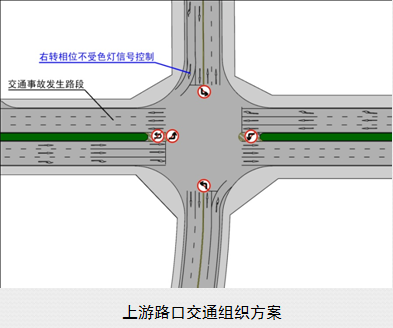
\includegraphics[width=.6\textwidth]{fig2}
\caption{上游路口交通组织方案}
\end{figure}

与此同时,在处于第一相位的30s内,来车量的也并非服从简单的均匀分布。观察视频我们可以看到,在第二相位期间,上游来车流量全部累积到路口,形成排队通过路口的车队;当红灯变为绿灯时,这些累积的车辆在短时间内释放,正面来车流量快速上升至一个很大的值,然后慢慢变小恢复到正常值。下面我们就具体的分析这一过程中的流量变化。

我们考察红灯线位置截面的车流流量。由定义我们可以直接得到,车流流量$q\left(x, t\right)$由车流密度$\rho \left(x, t\right)$和车流速度$v(x, t)$共同决定.$^{[2]}$:
\[
q\left( x,t \right)=\rho \left( x,t \right)v\left( x,t \right)
\]
$v\left( x,t \right)=$时,车流密度达到最大,$\rho \left( x,t
\right) {=}\rho_{max}$;当$\rho \left( x,t
\right) {=0}$时,车流速度达到最大,$v\left( x,t
\right)=v_{max}$。这两种情况我们称为平衡状态,而在非平衡状态下,根据文献.()(晏启鹏
2000)中的分析我们可以得到车流流量与车流密度的关系是:
\begin{equation}
q\left( \rho \right)=v_{max}\rho \left( 1-\frac{\rho }{\rho_{max}} \right)
\end{equation}
我们的目的是要描述车流流量 $ { }q $在红灯变为绿灯之后的时间段内随时间的变化过程,已经车流流量
$q$ 是关于 车流密度$ \rho $ 的函数,我们只需要分析车流密度 $\rho $
随时间的变化过程即可。

由定义,最大车流密度是车流速度为,车流平均车距为时的车流密度在,则此时道路空间的体积全部被车辆本身的体积占据。假设车流中车辆的平均长度为$d$,车辆的平均车距为$l$,那么我们可以得到公式:
\begin{equation}
\frac{\rho_{max}}{\rho }=\frac{l+d}{d}
\end{equation}

分析红灯变为绿灯后平均车距的变化。变为绿灯后,最靠前的车辆开始加速,与后面的车辆车距拉大,经过 \quad $\Delta
t $的时间后,后面的车辆同样开始加速;我们假设车辆从开始加速到达到最大速度经历一个匀加速过程,因此我们近似认为平均车距$l$ 正比于时间$t$:
\begin{equation}
l=kt
\end{equation}

我们联立III,IV和V得到:
\begin{equation}
q\left( t \right)=v_{max}\rho_{max}\frac{d}{kt+d}(1-\frac{d}{kt+d}) t\leq
t_{0}\end{equation}

注意到,公式VI描述的是排队车辆形成的密集车辆阵内的车流密度,那么,当这个车辆阵完全穿过指定横截面时,车流密度会发生一个瞬时的下降。由于正面来车流量在不考虑信号灯的条件下是一个常值
$q_{d}$, $q(t)$
将下降到这一常值后保持稳定。这样我们就得到了第一相位的一个30s周期内正面来车流量的变化规律(已将系数简化):
\begin{equation}
q_{d}\left( t \right)=\begin{cases}
aq_{d}\cdot \frac{1}{mt+1}(1-\frac{1}{mt+1}) &t\leq t_{a}\\
{q}_{d} &t>t_{a} \\
\end{cases}
\end{equation}

在使用matlab进行数值模拟时我们发现,如果直接采用公式VII进行模拟,由于模拟采用的离散值,而该函数在曲线阶段均为凸函数,且斜率变化较大,因此会出现明显的偏小的误差------实际模拟中正面车流流量的均值将小于连续函数给出的车流流量均值。因此我们采取阶梯函数近似的办法来描述第一相位时车流流量随时间的变化规律:
\begin{equation}
q_{d}\left( t \right)=\left( \chi_{\left[ 0,2 \right)}\left( t_{mod}
\right)\cdot  3+\chi_{\left[ 2,10 \right)}\left( t_{mod} \right)\cdot
5+\chi_{\left[ 10,12 \right)}\left( t_{mod} \right)\cdot  4+\chi_{\left[
12,30 \right)}\left( t_{mod} \right)\cdot  1 \right)\cdot
\frac{60}{72}\cdot  \tilde{q_{d}}(t)
\end{equation}
\begin{figure}[h]
\centering
\begin{minipage}{.45\textwidth}
\centering
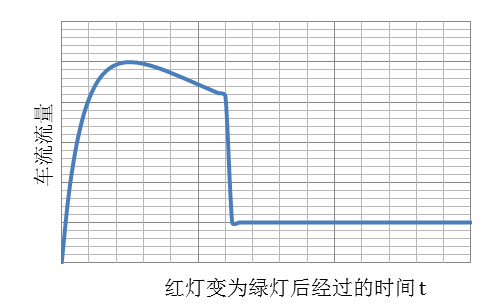
\includegraphics[width=.95\textwidth]{fig31}
\end{minipage}\hfill
\begin{minipage}{.45\textwidth}
\centering
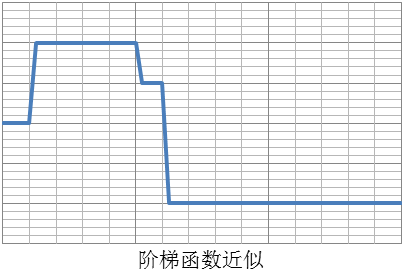
\includegraphics[width=.8\textwidth]{fig32}
\end{minipage}
\caption{上游路口交通组织方案}
\end{figure}

同时我们发现,不仅在一个周期内车流量变化存在明显的规则变化,在不同时间的不同周期内内的车流量也存在明显的变化。视频前部分的相位周期中周期总车流量较小,在视频后部分的相位周期中周期总车流量较大------这可能是由于下班晚高峰到来的影响。画出相位周期内平均车流流量随时间的变化,进行线性拟合,统计量
${R}^{{2}}=0.9196$,因此可以近似认为在研究时间段内单个周期总车流量呈线性增长:
\begin{equation}
\tilde{q_{d}}\left( t \right)= {\beta t+\gamma }
\end{equation}
\begin{figure}[h]
\centering
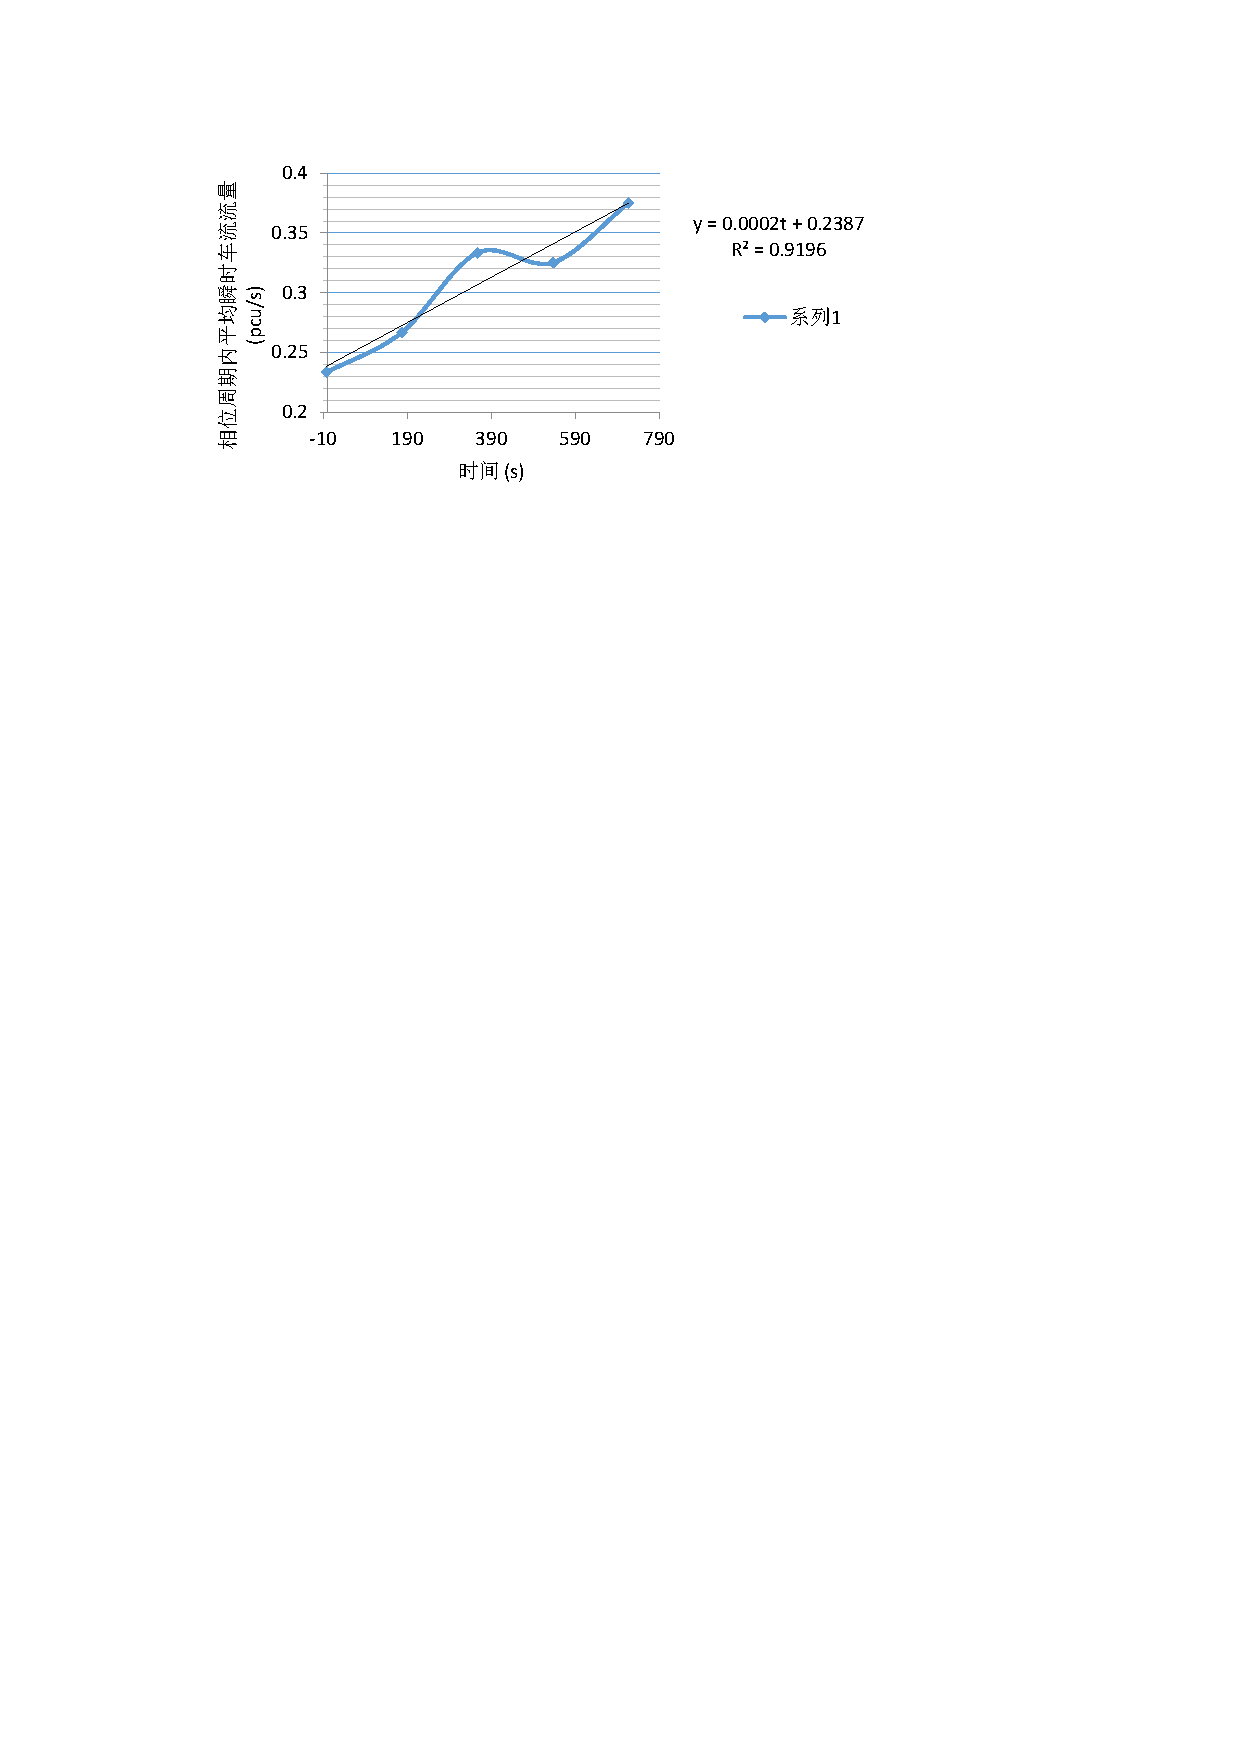
\includegraphics[width=.6\textwidth]{fig4}
\caption{前方来车相位周期内平均瞬时车流量的变化}
\end{figure}

加入第一相位和第二相位差别的考虑,我们得到最终的正面来车车流量的函数:
\begin{align}
{q_d}\left( t \right) =& \left( {\chi _{\left[ {0,2} \right)}}\left( {{t_{mod}}} \right)\cdot3 + {\chi _{\left[ {2,10} \right)}}\left( {{t_{mod}}} \right)\cdot5 + {\chi _{\left[ {10,12} \right)}}\left( {{t_{mod}}} \right)\cdot4+ {\chi _{\left[ {12,30} \right)}}\left( {{t_{mod}}} \right)\cdot1 \right)\nonumber\\
&\cdot\frac{{60}}{{72}}\left( {{ {\beta t}} + { {\gamma }}} \right)\cdot(1-\chi_{[30,60)} \cdot (t_mod ))
\end{align}
其中因子 $({1-\chi}_{\left[30,60 \right)})$ 含义是当${t}_{mod }\in \left[ 30,60 \right)$时,${q}_{d}=0$。

\subsubsection{路口右转来车流量}

由于上游的右转相位不受红色信号灯控制,故可认为右转来车是连续稳定的车流。同时统计显示右转来车相位周期内平均瞬时车流量随机震荡变化,没有明显的增减变化,故认为上游右转来车为常数值。

综合以上的讨论,将公式表格~2 和公式XII相加我们可以得到整个上游来车流量随时间的变化规律。

\subsection{参数估计}
根据图 4
前方来车相位周期内平均瞬时车流量的变化中Excel的回归分析,我们可以得到公式$\tilde{q_{d}}\left(
 {t} \right)$=$\beta $t$+\gamma $ IX的参数估计:
\[
\tilde{q_{d}}\left( t \right)=\beta t+\gamma =0.0002\cdot  t+0.2387
\]
公式中时间$ {t}$是指时间点到16:42:32的秒数差。如16:45:30对应的时间
$ {t=178 s}$。

我们统计了若干个相位周期右转来车的流量,得到了平均值为:
\[
\bar{q_{r}}=0.05 pcu/s
\]
\begin{table}[h]
\centering
\begin{tabular}{|p{85pt}|l|l|l|l|l|}
\hline
{开始时间}& {结束时间}& {小轿车}& {大客车}& {电瓶车}& {PCU} \\
\hline
16:42:00& 16:43:00& 2& & & 2 \\
\hline
16:45:00& 16:46:00& 3& & 1& 3.5 \\
\hline
16:47:00& 16:48:00& 2& & 3& 3.5 \\
\hline
16:50:00& 16:51:00& 1& & 1& 1.5 \\
\hline
16:53:00& 16:54:00& 4& & 1& 4.5 \\
\hline
\end{tabular}
\caption{上游右转来车流量统计}
\label{tab13}
\end{table}

然后考虑道路实际通行能力
$C$。在前面的讨论已经指出道路在饱和状态下的交通量即是道路实际通行能力的近似,我们统计了若干个饱和周期内的道路流量,计算出了视频1中事故位置横截面的道路实际通行能力:
\[
C=0.38062 pcu/s
\]
\begin{table}[h]
\centering
\begin{tabular}{|c|c|c|c|c|c|}
\hline
\textbf{开始时间}& \textbf{结束时间}& \textbf{小轿车}& \textbf{大客车}& \textbf{电瓶车}& \textbf{PCU} \\
\hline
16:42:32& 16:44:47& 27& 5& 5& 47 \\
\hline
16:47:58& 16:49:38& 33& 1& 8& 40.5 \\
\hline
16:52:42& 16:56:05& 91& 4& 17& 113.5 \\
\hline
\end{tabular}
\caption{上游正面来车流量统计}\label{tab14}
\end{table}

我们统计了$ {16:45:00}$到$ {16:58:00}$之间小区路口的车流变化,计算得到了两个小区路口进出车流的均值:
\begin{align*}
{XQ}_{1}\left( t \right)=\bar{{XQ}_{1}}=0.02083\  pcu/s\\
{XQ}_{2}\left( t \right)=\bar{{XQ}_{2}}=0.046474\  pcu/s
\end{align*}
我们还需要估计上游来车从路口到排队队伍末端的平均速度,观察视频我们给出估计值为:
\[
\hat{v}=10 m/s
\]
最后我们还需要确定比例常数 $ {\alpha
}$,即每$ {pcu}$的排队车辆所占的排队长度。我们截取了四张车辆排队图,统计各自的排队长度和排队标准车当量数,计算得到比例常数为:
\[
\alpha =4.8 m/pcu
\]
这样我们就得到视频1中该模型的所有参数。

\subsection{模型求解和分析}

利用我们分析得到的差分方程和估计得到的参数,我们可以解出排队长度随时间变化的关系。下面是由matlab解出的
$l-t$ 图:
\begin{figure}[h]
\centering
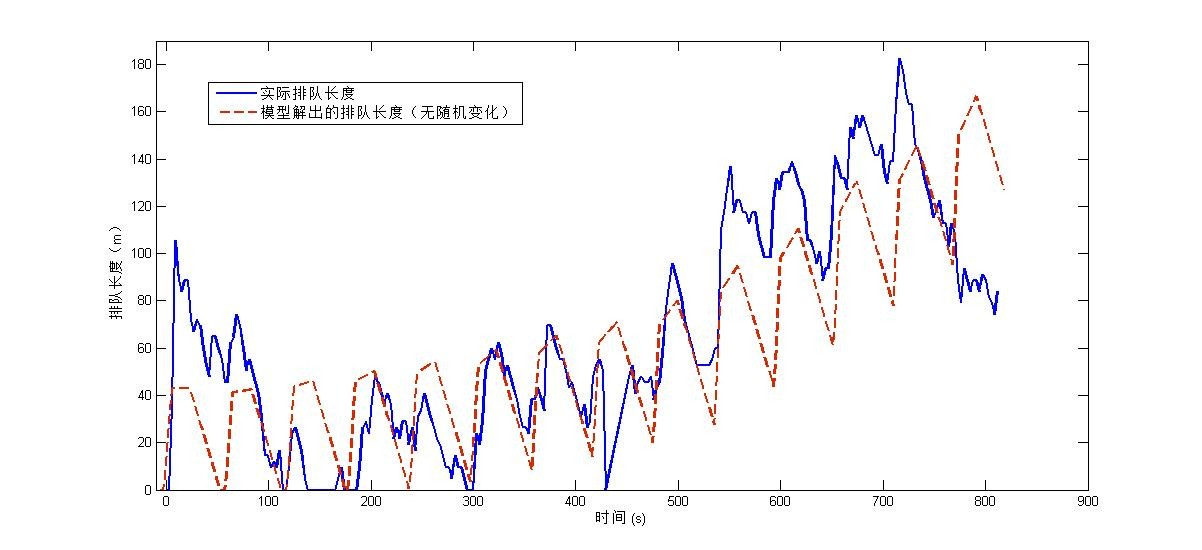
\includegraphics[width=.6\textwidth]{fig5}
\caption{未加入随机变化的模型解}
\end{figure}

观察图5,我们可以看到模型反映出,排队长度将在每个相位周期(60s)中震荡变化------这是因为进入第一相位后,上游车流急速上升,超过道路实际通行能力,因此排队长度迅速上升;而在离开第一相位,进入第二相位后,上游正面车流变为零,因此排队长度持续下降------模型很好地解释了排队长度的震荡变化。实际排队长度的变化表现出了更剧烈的上下震荡,但单位相周期内的平均排队长度依然有规律地随着时间增长,并且增长趋势和模型解是十分接近的。

\subsubsection{随机性的加入}
 
模型很好地解释了排队长度的大致变化趋势,但是由于现有模型中假设道路实际通行能力$C$,上游侧面车流量$q_{r},$小区车流${XQ}_{1}{XQ}_{2}$稳定不变以及排除信号灯作用的上游正面车流量$\tilde{q_{d}}$线性稳定变化,这和实际情况是有很大出入的。

显然,小区车流${XQ}_{1}{XQ}_{2}$和上游侧面车流量$q_{r}$都不是稳定不变,而是围绕平均值上下震荡的,有时会一次性来三四辆车,有时一分钟内到来的车仅一辆左右。同样,排除信号灯作用的上游正面车流量$\tilde{q_{d}}$虽然随时间大致呈线性增长的变化趋势,但实际情况依然是震荡上升的。最后,特别值得注意的是,道路实际通行能力$C$同样存在着随机的震荡,这是因为当车辆有序排队通过事故位置时,有较快的车速,而当不同车道的车流开始争抢通过事故位置时,就会出现短时的阻塞,车辆通过速度较慢。
\begin{figure}[h]
\centering
\begin{minipage}{.48\textwidth}
\centering
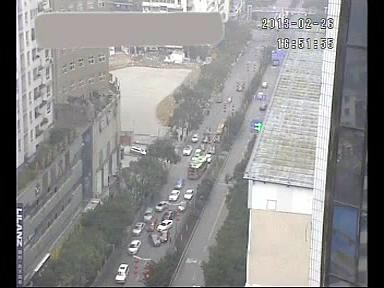
\includegraphics[width=.8\textwidth]{fig61}
\end{minipage}\hfill
\begin{minipage}{.48\textwidth}
\centering
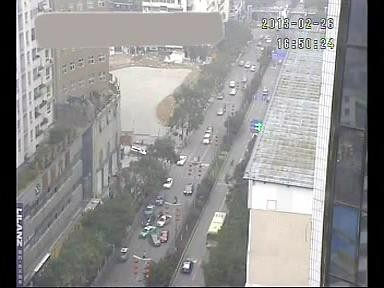
\includegraphics[width=.8\textwidth]{fig62}
\end{minipage}
\caption{有序高速通过(左图)和抢道低速通过(右图)}
\end{figure}


因此,要让我们的模型解更符合真实情况,我们必须将各个量的随机振动纳入模型。我们使用卡方分布$ {\chi
}^{ {2}}$描述这些随机量的震荡。由于$\tilde{q_{d}} {,}q_{r} {,}{XQ}_{1}{XQ}_{2}$这四个车流量的变化较为剧烈,我们假设它们服从均匀分布,即
\[
\tilde{q_{d}}\sim \bar{\tilde{q_{d}}}U_{\left[ 0,2 \right]}, q_{r}\sim
\bar{q_{r}}U_{\left[ 0,2 \right]}, {XQ}_{1}\sim \bar{{XQ}_{1}}U_{\left[ 0,2
\right]}, {XQ}_{2}\sim \bar{{XQ}_{2}}U_{\left[ 0,2 \right]}
\]
道路实际通行能能力的变化相对较小,我们假设它满足自由度为5的卡方分布,即:
\[
C\sim \bar{C}\frac{\chi^{2}\left( 5 \right)}{5}
\]
由于随机性的加入,每次模型求解得出的排队长度变化规律不尽相同,下图列举其中一些不同的排队长度变化情况,图中红色虚线表示实际排队长度。

通过上面两幅图我们可以看到加入了随机变化的模型解形态变化更加不规则,波动幅度更大,更加符合实际中排队长度的变化;同时在诸多随机模型解中也出现了一定比例的和实际排队长度非常接近的模型解。可以认为随机变化的加入是符合实际的。

\subsubsection{误差分析}
 
Matlab数值实验显示正面来车流量是决定排队长度的最重要因素,合理的秒数正面来车流量的变化是成功建模的关键。在该差分方程模型中,我们已经充分考虑相位周期内由于交通信号灯导致的流量变化和几个相位周期之间由于晚高峰到来导致的变化,在大部分时间段中,模型解都和实际排队长度符合的很好,但在$ {0\sim
60s}$ 和 $ {750s\sim 810}$s
两个相位周期内模型解和实际值偏差始终非常大。观察视频我们发现是这两个相位周期中上游来车流量偏离我们的线性估计很远------$ {0\sim
60s}$中的上游正面来车流量十分大,而$ {750s\sim
810}$s十分小。这说明我们的线性估计是不能完全合理描述相位周期间正面来车流量的变化,但由于偏离的混沌性和数据的有限性,做出更好估计的难度较大。

\subsubsection{控制变量分析}
 

除去时间参数$ {t}$外,模型中还有两个主要的自变量是道路通行能力$ {C}$和上游正面来车流量$q_{d}$,我们固定二者之一不变,那么排队长度就变成了关于时间参数$ {t}$和另一变量的函数,因此可以做出三维图分析其变化规律。

固定道路实际通行能力,我们看到在任何一个上游来车流量值下,排队长度依然呈现震荡变化;在上游来车流量较小时,道路通行能力能够释放所有的来车,因此每个相位周期后排队长度都能减小为零,而当上游来车流量较大时,道路通行能力不足以释放所有的来车,因此排队长度不断振荡上升。固定上游来车流量后的排队长度的变化类似。

为了获得排队长度和自变量更细致的关系,我们固定时间$ {t=800s}$,分析排队长度随时间的变化规律。

当道路通行能力固定时,我们看到排队长度随上游来车流量线性增长,Origin得出线性分析的统计量
$ {R}^{ {2}} {=0.97872}$,非常接近1,说明线性关系非常明显。

同样我们固定上游来车流量,分析排队长度随道路通行能力的变化规律。观察图形我们看到排队长度与道路通行能力呈现反相关关系,我们使用Origin执行指数回归分析得到统计量$R^{2}=0.9746$,非常接近1,说明负指数关系非常明显。

综合以上的分析,我们总结控制变量条件下,排队长度 $l$ 和事故发生时间
$ {t}$,道路通行能力$ { C}$ 以及上游来车流量 $ {q}$
之前的关系:


\subsection{模型评价}
\subsubsection{模型优点}
1)	差分方程结构简单,易于求解,计算复杂度低;

2)	对每个相位周期内正面来车流量的变化进行了非常细致的分析,把握住了影响排队长度的核心因素;

3)	模型参数较少,易于进行对实际情况的模拟。

\subsubsection{模型缺点}
1)	直接认为排队长度正比于排队车当量数,未考虑不同密度的排队车辆队伍;

2)	模型可能出现车流量可取任何连续值,不符合车辆数为离散整数的实际情况。
















\begin{thebibliography}{10}
\bibitem{1} \url{http://bbs.chinatex.org}
\bibitem{2} \url{http://www.chinatex.org}
\bibitem{3} Alpha Huang, \textbf{latex-notes-zh-cn}, 2014.
\bibitem{lf}M.R.C. van Dongen,\textbf{\LaTeX-and-Friends}, 2013.
\bibitem{figure}Keith Reckdahl,\textbf{Using Import graphics in \LaTeXe}, 1997.
\bibitem{HM}Addison Wesley,\textbf{Higher Mathematics}, 下载地址如下\\ \url{http://media.cism.it/attachments/ch8.pdf}
\end{thebibliography}


\newpage
\appendix
\section*{附 \quad 录}


\end{document}
